\documentclass[unicode, 8pt]{beamer}
\usetheme{Madrid}
\usecolortheme{seahorse}     %цветовая схема
\useinnertheme{circles}   %внутренняя тема
\usefonttheme{serif}    %шрифты

\usepackage[utf8]{inputenc}
\usepackage[T2A]{fontenc}
\usepackage[russian]{babel}
\usepackage[listings,theorems]{tcolorbox}
\usepackage{caption}
\usepackage[labelsep=period]{caption}
\setbeamertemplate{caption}[numbered]
\graphicspath{{../pic}}

\definecolor{shBlue}{HTML}{d6d6f0}
\definecolor{lightGray}{HTML}{F5F5F5}
\definecolor{spGreen}{HTML}{93DDC2}
\definecolor{spBlue}{HTML}{007AFF}
\definecolor{mainBackground}{HTML}{F9FEFC}

\makeatletter
\newcommand*{\rom}[1]{\expandafter\@slowromancap\romannumeral #1@}
\makeatother

\newcommand{\picref}[1]{рис. \ref{#1}}
\newcommand{\half}{\frac{1}{2}}
\newcommand{\dhalf}{\dfrac{1}{2}}
\newcommand*{\Scale}[2][4]{\scalebox{#1}{$#2$}}


\setbeamercolor{block title}{bg=shBlue!70,fg=black}
\setbeamercolor{block body}{bg=lightGray!50,fg=black}
% \setbeamercolor{frametitle}{fg=selected,bg=spGreen}
% \setbeamercolor{background canvas}{bg=mainBackground}
\setbeamertemplate{blocks}[rounded][shadow=false]

\title[Курсовая работа]{Кусочно-параболический метод на локальном шаблоне для решения линейного уравнения переноса}
\author[Токарев А.\,И.]{Выполнил: Токарев~А.\,И.\\[1ex]  {Научный руководитель: к. ф.-м. н., доц. каф. ФН2 Лукин~В.\,В.}}
\institute[]{МГТУ им. Н.Э. Баумана}
\date{\today}

\begin{document}

    \begin{frame}
        \titlepage
    \end{frame}

    \begin{frame}
        \frametitle{Содержание}
        \tableofcontents
    \end{frame}

    \section{Постановка задачи}

    \begin{frame}{Постановка задачи}
        \begin{block}{Линейное уравнение переноса}
         \begin{equation}
             \label{convection-diffusion}
             \dfrac{\partial y}{\partial t} + a \dfrac{\partial y}{\partial x} = 0.
         \end{equation}
        \end{block}

        \begin{block}{Характеристики}
            Характеристикой уравнения \eqref{convection-diffusion} является множество точек $(x,t)$, удовлетворяющее уравнению:
            \begin{equation}
                \label{characteristics}
                \dfrac{dx}{dt} = a,    
            \end{equation}
            \noindent то есть множество $x-at = b$. Таким образом, вдоль характеристики выполняется следующее равенство:
            \[
                \dfrac{dy}{dt} = 0.  
            \]
        \end{block}
        \begin{block}{Точное решение}
            Точное решение линейного уравнения переноса \eqref{convection-diffusion} представляется в виде:
            \[ y(x, t) = y_0(x-at), \]
            \noindent где $ y_0 $ -- начальный профиль.
        \end{block}
    \end{frame}

    \begin{frame}{Постановка задачи}
        \begin{block}{Задача Коши (начальная задача)}
            \begin{equation}
                \label{Cauchy}
                \Scale[0.9]  {
                    \begin{cases}
                        \,\dfrac{\partial y}{\partial t} + a \dfrac{\partial y}{\partial x} = 0, & x \in (-\infty,\, +\infty),\quad t > 0,
                        \\[1em]
                        \,y(x, 0) = y_0(x).
                        \\
                    \end{cases}
                }
            \end{equation}
            Решение задачи \eqref{Cauchy} заключается в сносе неизменного профиля по характеристикам. Его свойством является сохранение начального профиля $y_0$.
        \end{block}

        \begin{block}{Сетка}
            Введем сетку, на которой будем решать задачу:
            \[
                \Omega_h = \Bigl\{ x_i = l_1 + i h,\,\, i = 1 \ldots n,\,\, h = \frac{l_2-l_1}{n-1} \Bigr\},
            \]
            где $[l_1, l_2]$ -- отрезок, на котором определена сетка; $n$~--~число узлов; $h$ -- шаг. Определим $y(x)$ ее разностным аналогом $y_i=y(x_i)$ на этой сетке. Значения $y_i$ будем соотносить с \\[0.3em] узлами сетки, а $ y_{ i + \half} = y_i^R $ и $ y_{i - \half} = y_i^L $ -- с половинными узлами.
        \end{block}
    \end{frame}

    \begin{frame}{Интегро-интерполяционный метод. Перенос узлов}
        Определив решения $y_i$ в момент времени $ t_j $, можно вычислить $ \hat y_i $ на следующем временном слое $ t_{j+1} $, применив интегро-интерполяционный метод к уравнению переноса в прямоугольнике $ \bigl[ x_{i-\half}, x_{i+\half} \bigr] \times [t_j, t_{j+1}] $:
        \[
            \displaystyle \int \limits_{x_{i-\half}}^{x_{i+\half}} \int \limits_{t_j}^{t_{j+1}} \dfrac{ \partial y(x, t) }{ \partial t } \, dt \, dx \,\, + \int \limits_{t_j}^{t_{j+1}} \int \limits_{x_{i-\half}}^{x_{i+\half}} a \dfrac{ \partial y(x,t) }{ \partial x } \, dx \, dt \,\, = \int \limits_{x_{i-\half}}^{x_{i+\half}} \int \limits_{t_j}^{t_{j+1}} 0 \, dt \, dx \, \, = 0.
        \]
        Рассмотрим интегралы по отдельности: 
        \[
            \begin{split}
                \int \limits_{x_{i-\half}}^{x_{i+\half}} \int \limits_{t_j}^{t_{j+1}} \dfrac{ \partial y(x, t) }{ \partial t } \, dt \, dx \,\, &= \int \limits_{x_{i-\half}}^{x_{i+\half}} \Bigl[ y(x, t_{j+1}) - y(x, t_j)  \Bigr] \, dx = h \Bigl[ \dfrac{1}{h} \int \limits_{x_{i-\half}}^{x_{i+\half}} y(x, t_{j+1}) \, dx \,\,  -  
                \\ 
                &- \dfrac{1}{h} \int \limits_{x_{i-\half}}^{x_{i+\half}} y(x, t_j) \, dx \Bigr] = h ( \overline y(x_i, t_{j+1}) - \overline y(x_i, t_j) ) = h( \hat y_i - y_i).
            \end{split}
        \]
    \end{frame}
 
     \begin{frame}{Интегро-интерполяционный метод. Перенос узлов}
        Воспользуемся особенностью переноса значений по характеристикам для интеграла, подинтегральная функция которого является потоком (\picref{fig:flow_visual}):
        \[
            \begin{split}
                \int \limits_{t_j}^{t_{j+1}} \int \limits_{x_{i-\half}}^{x_{i+\half}} a \dfrac{ \partial y(x,t) }{ \partial x } \, dx \, dt \,\, &= \int \limits_{t_j}^{t_{j+1}} a \bigl( y(x_{i+\half}, t) - y(y_{x-\half}, t) \bigr) \, dt \,\, =  \int \limits_{x_{i+\half}-a\tau}^{x_{i+\half}} a y(x, t_j) \, dt \,\, - \\
                &- \int \limits_{x_{i-\half}-a\tau}^{x_{i-\half}} a y(x, t_j) \, dt = a\tau\bigl( a \overline y_{i+\half} - a \overline y_{i-\half} \bigr).
            \end{split}
        \]
        Объединяя оба интеграла получаем:
        \begin{equation}
            \begin{split}
                h ( \hat y_i - y_i) &+ a\tau\bigl( a \overline y_{i+\half} - a \overline y_{i-\half} \bigr) = 0 \,\, \Rightarrow \,\, \hat y_i = y_i - \dfrac{ a\tau }{ h } \Bigl( a \overline y_{i+\half} - a \overline y_{i-\half} \Bigr).
            \end{split}
            \label{center}
        \end{equation}
        В соответствии с формулой \eqref{center} переносятся значения в узлах сетки $ y_i = y(x_i)$ на следующий временной слой.
     \end{frame}
 
     \begin{frame}
         \begin{figure}[h]
             \centering
             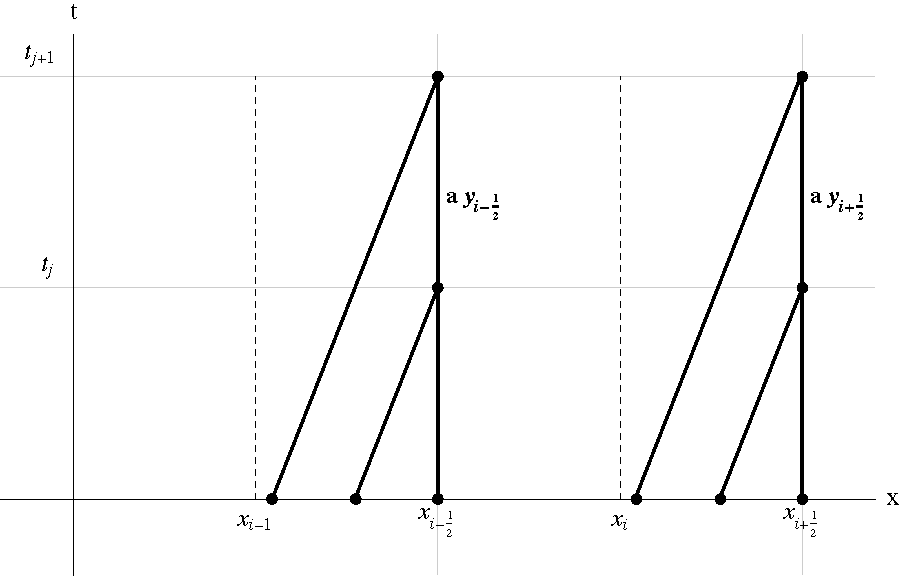
\includegraphics[width=0.95\textwidth]{flow_visual.pdf}
             \caption{Интегрирование потока по пространству, вместо времени}
             \label{fig:flow_visual}
         \end{figure}
     \end{frame}

    \section{Методы решения}
    \begin{frame}{Методы решения}
        \begin{block}{Общая идея}
            Имея значения в узлах $x_i,\, i = 0 \ldots n$, доопределяем значения в половинных узлах, то есть исходная сетка $\Omega_h$ преобразуется в набор отрезков $\bigl[ x_{i-\half}, x_{i+\half} \bigr]$ с определенными в них параболами (\picref{fig:ppm_visual}):
            \begin{equation}
                \label{parabolic_eq}
                \begin{split}
                    &y(x) = y_i^L + \xi(\Delta y_i + y_i^{(6)}(1 - \xi)), \quad \xi = (x - x_{i-\half})h^{-1}, \quad  \Delta y_i = y_i^R-y_i^L, 
                    \\
                   &y_i^{(6)} = 6\Bigl[ y_i - \half(y_i^R + y_i^L)\Bigr], \quad x \in [x_{i-\half}, x_{i + \half}]. 
                \end{split}
            \end{equation}
        \end{block}

        \begin{figure}[h]
            \centering
            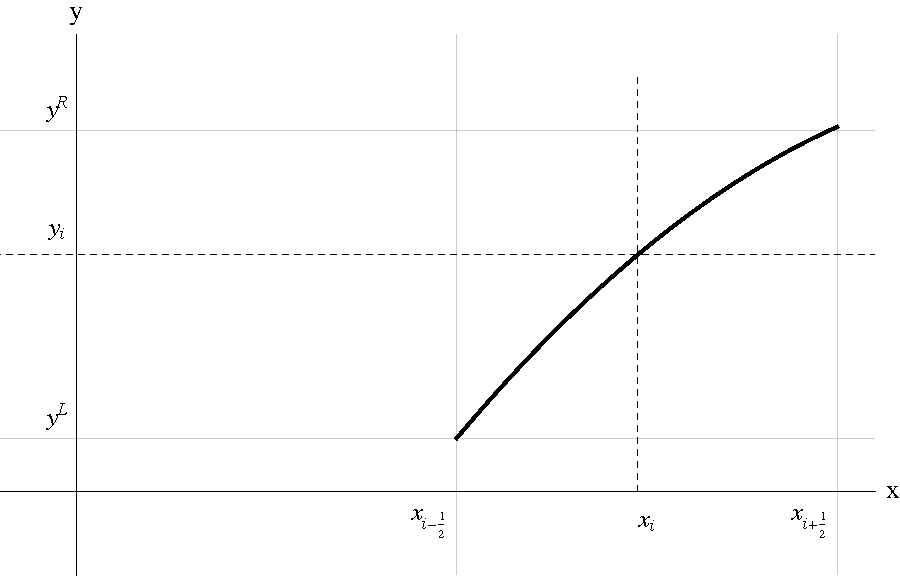
\includegraphics[width=0.47\textwidth]{ppm_visual.pdf}
            \caption{Парабола внутри разностной ячейки}
            \label{fig:ppm_visual}
        \end{figure}
    \end{frame}

    \begin{frame}{Средние значения на отрезке}
        Для выражение \eqref{parabolic_eq} выполняется соотношение:
            \begin{equation}
                \label{average}
                \Scale[0.9] {
                    y(x_i) = \dfrac{1}{h} \displaystyle \int\limits_{x_{i-\half}}^{x_{i+\half}} y(\chi) d\chi,
                }
            \end{equation}
            \noindent то есть значения в узлах сетки $\Omega_h$ являются средними значениями.

        \begin{block}{Среднее значение на отрезке}
            После определения парабол можно считать средние значения на отрезках $ [x_{i+\half}-\alpha, x_{i+\half}] $ и $ [x_{i+\half}, x_{i+\half}+\alpha]\colon $
            \begin{equation}
                \label{average_positive}
                \Scale[0.9] {
                    \overline y_{i+\half}^L(\alpha) = \dfrac{1}{\alpha} \displaystyle \int\limits_{x_{i+\half}-\alpha}^{x_{i+\half}} y(x) dx = y_i^R - \dfrac{\alpha}{2h}\Bigl[ \Delta y_i - \Bigl( 1 - \dfrac{2 \alpha}{3h} \Bigr)y_i^{(6)} \Bigr],
                }
            \end{equation}
            \begin{equation}
                \label{average_negative}
                \Scale[0.9] {
                    \overline y_{i+\half}^R = \dfrac{1}{\alpha} \displaystyle \int\limits_{x_{i+\half}}^{x_{i+\half}+\alpha} y(x) dx = y_{i+1}^L  + \dfrac{\alpha}{2h} \Bigl[\Delta y_{i+1} + \Bigl( 1 - \dfrac{2\alpha}{3h} \Bigr) y_{i+1}^{(6)} \Bigr].
                }
            \end{equation}
        \end{block}
    \end{frame}

    \begin{frame}{Кусочно-параболические методы. PPM и PPML}
        \begin{block}{Граничные значения в PPM}
            \[
                y_i^R = y_{i+1}^L = y_{i+\half} = \dhalf(y_i + y_{i+1}) - \dfrac{1}{6}(\delta y_{i+1} - \delta y_i), \quad \delta y_i = \dhalf(y_{i+1} + y_{i-1}).
            \]
            Для того, чтобы обеспечить монотонность решения, $\delta y_i$ заменяется на:
            \[
                \Scale[0.95] {
                    \delta_m y_i = 
                    \begin{cases}
                        \min(|\delta y_i|,\, 2|y_i - y_{i-1}|,\, 2|y_{i+1} - y_i|)\cdot sign(\delta y_i), & (y_{i+1} - y_i)(y_i - y_{i-1}) > 0, \\
                        0, \quad (y_{i+1} - y_i)(y_i - y_{i-1}) \leq 0.
                    \end{cases}   
                } 
            \]
        \end{block}

        \begin{block}{Граничные значения в PPML}
            В качестве альтернативы предлагает перенос граничных узлов по характеристикам. \\[0.5em] Пусть $ \frac{dx}{dt} = a $.
            \begin{itemize}
                \item Если $ a > 0 $, то получаем:
                \[
                    \Scale[0.95] {
                        y_{i+\half}(t_{j+1}) = y_i^R(t_{j+1}) = y_i^L(t_j) + \xi(\Delta y_i(t_j) + y_i^{(6)}(t_j)(1-\xi)), \quad \xi = 1 -  \dfrac{a \tau}{h}.
                    }
                \]        
                \item При $ a < 0 $:
                \[
                    \Scale[0.95] {
                        y_{i+\half}(t_{j+1}) = y_i^R(t_{j+1}) = y_{i+1}^L(t_j) + \xi(\Delta y_{i+1}(t_j) + y_{i+1}^{(6)}(t_j)(1-\xi)), \quad \xi = -\dfrac{a \tau}{h}.
                    }
                \]
            \end{itemize}
        \end{block}
    \end{frame}

    \begin{frame}{Монотонизация}
        \begin{figure}[h]
            \centering
            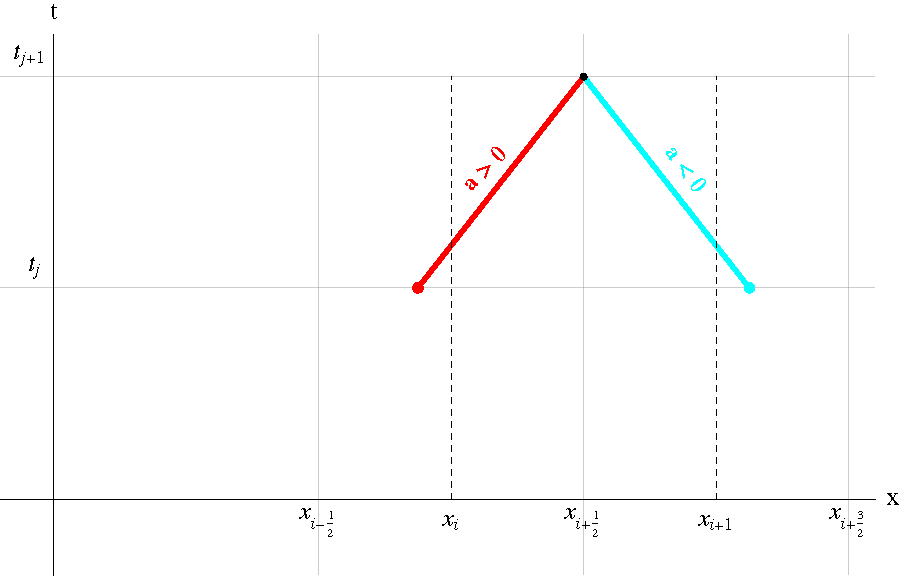
\includegraphics[width=0.4\textwidth]{ppml_visual.pdf}
            \caption{Перенос значений на границах вдоль характеристик в методе PPML}
            \label{fig:ppml_visual}
        \end{figure}
        \begin{block}{Избавление от локальных экстремумов}
            \begin{itemize}
                \item $ y_i $ является локальным экстремумом, тогда:
                \[
                    y_i^L = y_i^R = y_i, \quad (y_{i+1} - y_i)(y_i - y_{i-1}) \leq 0;
                \]       
                \item $ y_i $ лежит слишком близко к границе:
                \[
                    \begin{split}
                        y_i^L = 3y_i -2y_i^R, &\quad \Delta y_i \cdot y_i^{(6)} > (\Delta y_i)^2, \\
                        y_i^R = 3y_i -2y_i^L, &\quad \Delta y_i \cdot y_i^{(6)} < -(\Delta y_i)^2.
                    \end{split}  
                \]
            \end{itemize}
        \end{block}
    \end{frame}

    \section{Тестирование и сравнение методов}
    \begin{frame}{Тестирование и сравнение методов}
        \begin{block}{Нормы ошибок решения в различных пространствах}
            Норма ошибка в пространстве $C\colon$
            \[
                \Scale[0.97]{
                    \|z\|_{C} = \max_{\Omega_h \times [0, T]} |z|, \quad z = |y(x,t)-y_h(x,t)|.
                }
            \]
            Норма ошибка в пространстве $L_1\colon$
            \[
                \Scale[0.97]{
                    \|z\|_{L_1} = \displaystyle \int\limits_{0}^{T}\int\limits_{\Omega_h} |z|\, dx dt, \quad z = |y(x,t)-y_h(x,t)|.
                }
            \]
            Норма ошибка в пространстве $L_2\colon$
            \[
                \Scale[0.97]{
                    \|z\|_{L_2} = \Biggl( \displaystyle \int\limits_{0}^{T}\int\limits_{\Omega_h} z^2\, dx dt \Biggr)^{\tfrac{1}{2}}, \quad z = |y(x,t)-y_h(x,t)|.
                }
            \]
        \end{block}
        \begin{block}{Исходные параметры}
            Рассмотрим несколько начальных профилей [3] и проанализируем точность каждого из методов в различных сценариях. Примем $ l = 200,\, l_1 = 10,\, l_2 = 30, l_{11} = \frac{50}{3}, l_{22} = \frac{70}{3},$
            \noindent$ l_{12} = 20,\, T = 200,\, h = 1,\, a = 1$.
        \end{block}
    \end{frame}

    \begin{frame}{Анализ точного вычисления граничных и серединных узлов}
        \begin{figure}[h]
            \centering
            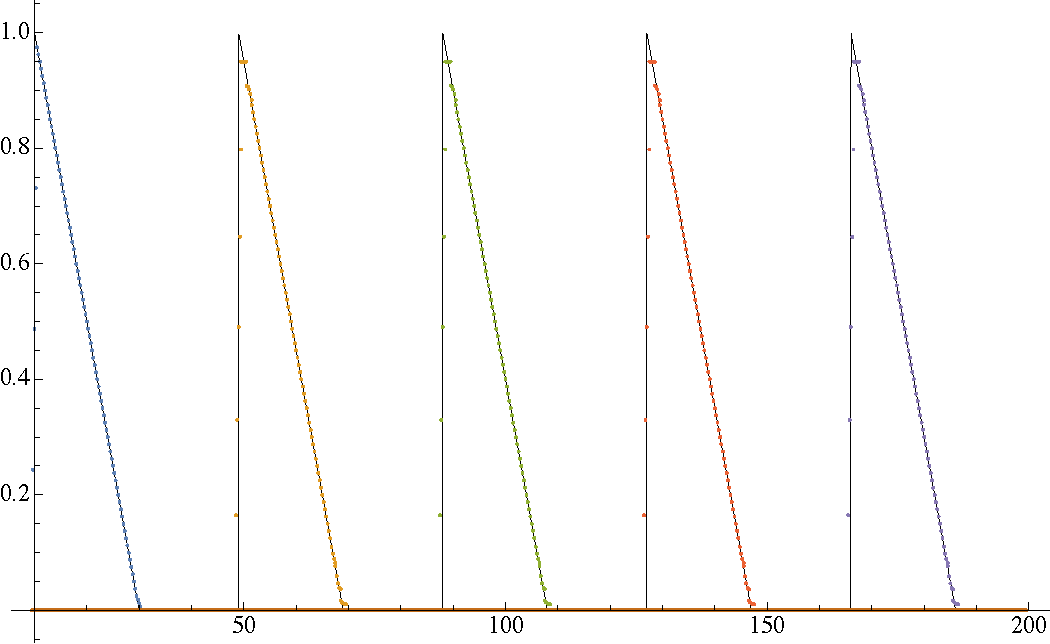
\includegraphics[width=0.66\textwidth]{sigma=1./advectionPPM_rightTriangle.pdf}
            \caption{Правый треугольник для PPM при $ \sigma = 1 $}
            \label{fig:ppm_rightTriangle_1}
        \end{figure}
        \begin{table}[h]
            \centering
            \begin{tabular}{ |c|c|c|c|c|c| } 
             \hline
              & $ h=1 $ &  $ h=0.5$ &  $ h=0.25 $ &  $ h=0.125 $ &  $ h=0.0625 $ \\ 
             \hline
             $\| \cdot \|_{C}$ & $0.5125$ & $0.506$ & $0.503$ & $0.501$ & $0.5$
             \\
             \hline
             $\| \cdot \|_{L_1}$ & $25.6$ & $6.32$ & $1.57$ & $0.39$ & $0.1$
             \\
             \hline
             $\| \cdot \|_{L_2}$ & $2.89$ & $1.44$ & $0.72$ & $0.36$ & $0.18$ \\
             \hline 
            \end{tabular}
            \\[0.1em]
            \caption{Нормы ошибок для правого треугольника в методе PPM}
            \label{table:ltPPM}
        \end{table}
    \end{frame}

    \begin{frame}{Анализ точного вычисления граничных и серединных узлов}
        \begin{figure}[h]
            \centering
            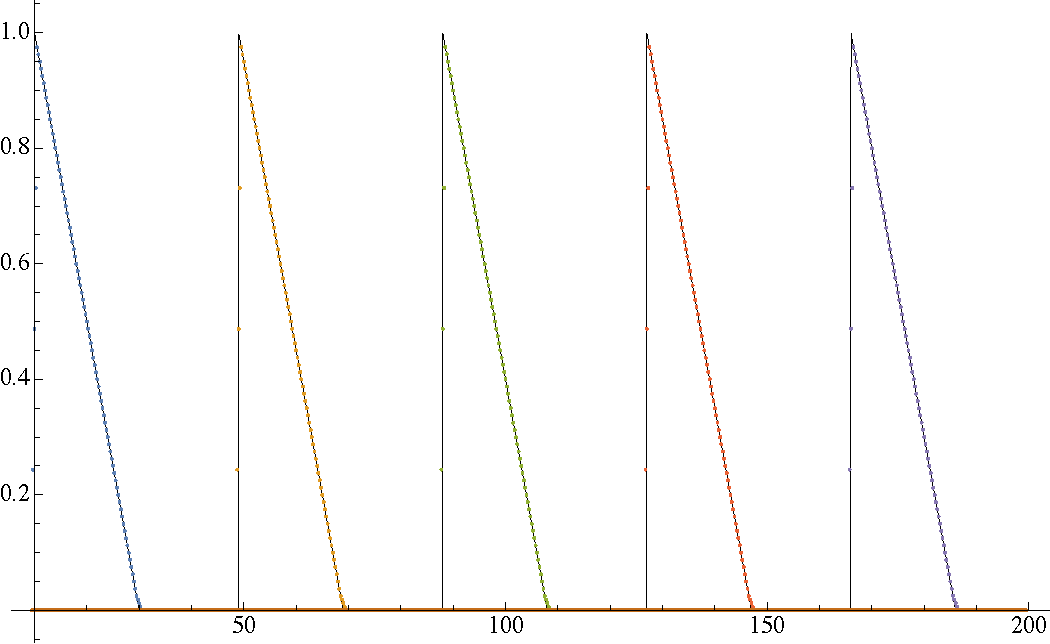
\includegraphics[width=0.66\textwidth]{sigma=1./advectionPPML_rightTriangle.pdf}
            \caption{Правый треугольник для PPML при $ \sigma = 1 $}
            \label{fig:ppml_rightTriangle_1}
        \end{figure}
        \begin{table}[h]
            \centering
            \begin{tabular}{ |c|c|c|c|c|c| } 
             \hline
            & $ h=1 $ &  $ h=0.5$ &  $ h=0.25 $ &  $ h=0.125 $ &  $ h=0.0625 $ \\ 
             \hline 
             $\| \cdot \|_{C}$ & $0.5125$ & $0.505$ & $0.5029$ & $0.5025$ & $0.5$
             \\
             \hline
             $\| \cdot \|_{L_1}$ & $25.6$ & $6.32$ & $1.57$ & $0.39$ & $0.1$
             \\
             \hline
             $\| \cdot \|_{L_2}$ & $2.86$ & $1.42$ & $0.71$ & $0.305$ & $0.17$
             \\
             \hline
            \end{tabular}
            \\[0.1em]
            \caption{Нормы ошибок для правого треугольника в методе PPML}
            \label{table:ltPPML}
        \end{table}
    \end{frame}

    \begin{frame}{Анализ кусочно-линейного графика при уменьшенном числе Куранта}
        \begin{figure}[h]
            \centering
            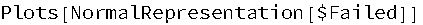
\includegraphics[width=0.6\textwidth]{sigma=0.8/advectionPPM_tooth.pdf}
            \caption{Зуб для PPM при $ \sigma = 0.8 $}
            \label{fig:ppm_tooth_08}
        \end{figure}
        \begin{table}[h]
            \centering
            \begin{tabular}{ |c|c|c|c|c|c| } 
             \hline
             & $ h=1 $ &  $ h=0.5$ &  $ h=0.25 $ &  $ h=0.125 $ &  $ h=0.0625 $ \\ 
             \hline 
             $\| \cdot \|_{C}$ & $0.716$ & $0.7099$ & $0.7067$ & $0.7023$ & $0.7$
             \\
             \hline
             $\| \cdot \|_{L_1}$ & $41.15$ & $10.14$ & $2.518$ & $0.62$ & $0.3$
             \\
             \hline
             $\| \cdot \|_{L_2}$ & $0.8$ & $0.39$ & $0.195$ & $0.097$ & $0.04$
             \\
             \hline
            \end{tabular}
            \\[0.1em]
            \caption{Нормы ошибок для профиля "зуб" в методе PPM}
            \label{table:toothPPM}
        \end{table}
    \end{frame}

    \begin{frame}{Анализ кусочно-линейного графика при уменьшенном числе Куранта}
        \begin{figure}[h]
            \centering
            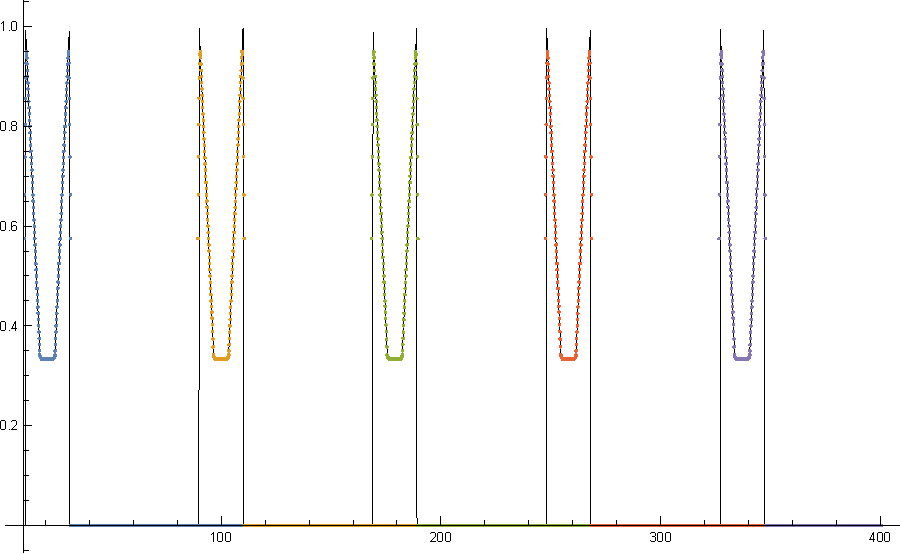
\includegraphics[width=0.6\textwidth]{sigma=0.8/advectionPPML_tooth.pdf}
            \caption{Зуб для PPML при $ \sigma = 0.8 $}
            \label{fig:ppml_tooth_08}
        \end{figure}
        \begin{table}[h]
            \centering
            \begin{tabular}{ |c|c|c|c|c|c| } 
             \hline
             & $ h=1 $ &  $ h=0.5$ &  $ h=0.25 $ &  $ h=0.125 $ &  $ h=0.0625 $ 
             \\ 
             \hline
             $\| \cdot \|_{C}$ & $0.58$ & $0.56$ & $0.557$ & $0.554$ & $0.55$ 
             \\
             \hline
             $\| \cdot \|_{L_1}$ & $39.85$ & $9.9$ & $2.2$ & $0.56$ & $0.27$
             \\
             \hline
             $\| \cdot \|_{L_2}$ & $0.7$ & $0.34$ & $0.187$ & $0.08$ & $0.03$ 
             \\
             \hline
            \end{tabular}
            \\[0.1em]
            \caption{Нормы ошибок для профиля "зуб" в методе PPML}
            \label{table:toothPPML}
        \end{table}
    \end{frame}

    \begin{frame}{Анализ методов на гладком графике}
        \begin{figure}[h]
            \centering
            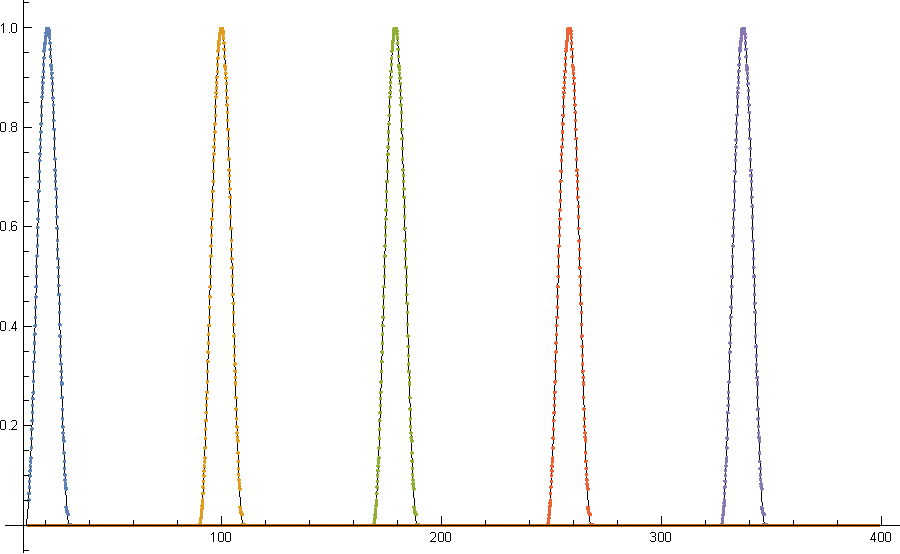
\includegraphics[width=0.6\textwidth]{sigma=0.5/advectionPPM_cos.pdf}
            \caption{Косинус для PPM при $ \sigma = 0.5 $}
            \label{fig:ppm_cos_05}
        \end{figure}
        \begin{table}[h]
            \centering
            \begin{tabular}{ |c|c|c|c|c|c| } 
             \hline
             & $ h=1 $ &  $ h=0.5$ &  $ h=0.25 $ &  $ h=0.125 $ &  $ h=0.0625 $ \\ 
             \hline
             $\| \cdot \|_{C}$ & $0.244$ & $0.1117$ & $0.044$ & $0.019$ & $1e{-05}$
             \\
             \hline
             $\| \cdot \|_{L_1}$ & $2.59$ & $0.327$ & $0.04$ & $0.005$ & $2e{-05}$
             \\
             \hline
             $\| \cdot \|_{L_2}$ & $0.99$ & $0.18$ & $0.003$ & $0.00055$ & $2e{-05}$ 
             \\
             \hline
            \end{tabular}
            \\[0.1em]
            \caption{Нормы ошибок для косинуса в методе PPM}
            \label{table:cosPPM}
        \end{table}    
    \end{frame}

    \begin{frame}{Анализ методов на гладком графике}
        \begin{figure}[h]
            \centering
            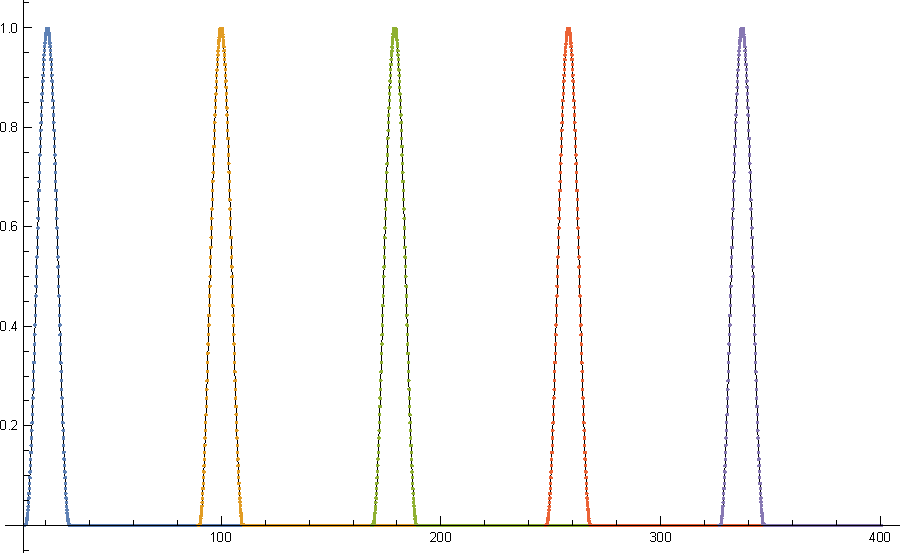
\includegraphics[width=0.6\textwidth]{sigma=0.5/advectionPPML_cos.pdf}
            \caption{Косинус для PPML при $ \sigma = 0.5 $}
            \label{fig:ppml_cos_05}
        \end{figure}
        \begin{table}[h]
            \centering
            \begin{tabular}{ |c|c|c|c|c|c| } 
             \hline
             & $ h=1 $ &  $ h=0.5$ &  $ h=0.25 $ &  $ h=0.125 $ &  $ h=0.0625 $ \\ 
             \hline
             $\| \cdot \|_{C}$ & $0.048$ & $0.015$ & $0.005$ & $0.0016$ & $1e{-06}$
             \\
             \hline
             $\| \cdot \|_{L_1}$ & $2.55$ & $0.32$ & $0.0398$ & $0.0049$ & $2e{-06}$
             \\
             \hline
             $\| \cdot \|_{L_2}$ & $0.99$ & $0.18$ & $0.003$ & $0.00055$ & $2e{-06}$ 
             \\
             \hline
            \end{tabular}
            \\[0.1em]
            \caption{Нормы ошибок для косинуса в методе PPML}
            \label{table:cosPPML}
         \end{table}
    \end{frame}

    \section{Заключение}
    \begin{frame}{Заключение}
        Рассмотрен кусочно-параболический метод на локальном шаблоне. Выбор в пользу использования решений с предыдущего временного слоя, вместо интерполяционной процедуры, оказался удачным, так как обеспечивает более точное решение и уменьшенную диссипацию. Метод PPML был протестирован на ряде примеров, рассмотренных с различными шагами, числами Куранта и профилями. Точность оценивалась на основе норм разности между точным и численным решениям в пространствах $ C,\, L_1,\, L_2 $. В пространствах $L_1, \, L_2$ PPML оказался точнее во всех случаях. Однако в пространстве $C$ результат нельзя интерпретировать однозначно. Но как уже отмечалось, актуальной является сходимость нормы ошибки в $L_2$.
    \end{frame}

\end{document}